\documentclass[ucs,9pt]{beamer}

% Copyright 2004 by Till Tantau <tantau@users.sourceforge.net>.
%
% In principle, this file can be redistributed and/or modified under
% the terms of the GNU Public License, version 2.
%
% However, this file is supposed to be a template to be modified
% for your own needs. For this reason, if you use this file as a
% template and not specifically distribute it as part of a another
% package/program, I grant the extra permission to freely copy and
% modify this file as you see fit and even to delete this copyright
% notice.
%
% Modified by Tobias G. Pfeiffer <tobias.pfeiffer@math.fu-berlin.de>
% to show usage of some features specific to the FU Berlin template.

% remove this line and the "ucs" option to the documentclass when your editor is not utf8-capable
\usepackage[utf8x]{inputenc}    % to make utf-8 input possible
\usepackage[english]{babel}     % hyphenation etc., alternatively use 'german' as parameter

% Template for talks using the Corporate Design of the Freie Universitaet
%   Berlin, created following the guidelines on www.fu-berlin.de/cd by
%   Tobias G. Pfeiffer, <tobias.pfeiffer@math.fu-berlin.de>
% This file can be redistributed and/or modified in any way you like.
%   If you feel you have done significant improvements to this template,
%   please consider providing your modified version to
%   https://www.mi.fu-berlin.de/w/Mi/BeamerTemplateCorporateDesign

\usepackage{amsmath,dsfont,listings}

%%% FU logo
% small version for upper right corner of normal pages
\pgfdeclareimage[height=0.9cm]{university-logo}{FULogo_RGB}
\logo{\pgfuseimage{university-logo}}
% large version for upper right corner of title page
\pgfdeclareimage[height=1.085cm]{big-university-logo}{FULogo_RGB}
\newcommand{\titleimage}[1]{\pgfdeclareimage[height=2.92cm]{title-image}{#1}}
\titlegraphic{\pgfuseimage{title-image}}
%%% end FU logo

% NOTE: 1cm = 0.393 in = 28.346 pt;    1 pt = 1/72 in = 0.0352 cm
\setbeamersize{text margin right=3.5mm, text margin left=7.5mm}  % text margin

% colors to be used
\definecolor{text-grey}{rgb}{0.45, 0.45, 0.45} % grey text on white background
\definecolor{bg-grey}{rgb}{0.66, 0.65, 0.60} % grey background (for white text)
\definecolor{fu-blue}{RGB}{0, 51, 102} % blue text
\definecolor{fu-green}{RGB}{153, 204, 0} % green text
\definecolor{fu-red}{RGB}{204, 0, 0} % red text (used by \alert)

% switch off the sidebars
% TODO: loading \useoutertheme{sidebar} (which is maybe wanted) also inserts
%   a sidebar on title page (unwanted), also indents the page title (unwanted?),
%   and duplicates the navigation symbols (unwanted)
\setbeamersize{sidebar width left=0cm, sidebar width right=0mm}
\setbeamertemplate{sidebar right}{}
\setbeamertemplate{sidebar left}{}
%    XOR
% \useoutertheme{sidebar}

% frame title
% is truncated before logo and splits on two lines
% if neccessary (or manually using \\)
\setbeamertemplate{frametitle}{%
    \vskip-30pt \color{text-grey}\large%
    \begin{minipage}[b][23pt]{80.5mm}%
    \flushleft\insertframetitle%
    \end{minipage}%
}

%%% title page
% TODO: get rid of the navigation symbols on the title page.
%   actually, \frame[plain] *should* remove them...
\setbeamertemplate{title page}{
% upper right: FU logo
\vskip2pt\hfill\pgfuseimage{big-university-logo} \\
\vskip6pt\hskip3pt
% title image of the presentation
\begin{minipage}{11.6cm}
\hspace{-1mm}\inserttitlegraphic
\end{minipage}

% set the title and the author
\vskip14pt
\parbox[top][1.35cm][c]{11cm}{\color{text-grey}\inserttitle \\ \small \insertsubtitle}
\vskip11pt
\parbox[top][1.35cm][c]{11cm}{\small \insertauthor \\ \insertinstitute \\[3mm] \insertdate}
}
%%% end title page

%%% colors
\usecolortheme{lily}
\setbeamercolor*{normal text}{fg=black,bg=white}
\setbeamercolor*{alerted text}{fg=fu-red}
\setbeamercolor*{example text}{fg=fu-green}
\setbeamercolor*{structure}{fg=fu-blue}

\setbeamercolor*{block title}{fg=white,bg=black!50}
\setbeamercolor*{block title alerted}{fg=white,bg=black!50}
\setbeamercolor*{block title example}{fg=white,bg=black!50}

\setbeamercolor*{block body}{bg=black!10}
\setbeamercolor*{block body alerted}{bg=black!10}
\setbeamercolor*{block body example}{bg=black!10}

\setbeamercolor{bibliography entry author}{fg=fu-blue}
% TODO: this doesn't work at all:
\setbeamercolor{bibliography entry journal}{fg=text-grey}

\setbeamercolor{item}{fg=fu-blue}
\setbeamercolor{navigation symbols}{fg=text-grey,bg=bg-grey}
%%% end colors

%%% headline
\setbeamertemplate{headline}{
\vskip4pt\hfill\insertlogo\hspace{3.5mm} % logo on the right

\vskip6pt\color{fu-blue}\rule{\textwidth}{0.4pt} % horizontal line
}
%%% end headline

%%% footline
\newcommand{\footlinetext}{\insertshortinstitute, \insertshorttitle, \insertshortdate}
\setbeamertemplate{footline}{
\vskip5pt\color{fu-blue}\rule{\textwidth}{0.4pt}\\ % horizontal line
\vskip2pt
\makebox[123mm]{\hspace{7.5mm}
\color{fu-blue}\footlinetext
\hfill \raisebox{-1pt}{\usebeamertemplate***{navigation symbols}}
\hfill \insertframenumber}
\vskip4pt
}
%%% end footline

%%% settings for listings package
\lstset{extendedchars=true, showstringspaces=false, basicstyle=\footnotesize\sffamily, tabsize=2, breaklines=true, breakindent=10pt, frame=l, columns=fullflexible}
\lstset{language=Java} % this sets the syntax highlighting
%\lstset{mathescape=true} % this switches on $...$ substitution in code
% enables UTF-8 in source code:
\lstset{literate={ä}{{\"a}}1 {ö}{{\"o}}1 {ü}{{\"u}}1 {Ä}{{\"A}}1 {Ö}{{\"O}}1 {Ü}{{\"U}}1 {ß}{\ss}1}
%%% end listings
  % THIS is the line that includes the FU template!

\usepackage{arev,t1enc} % looks nicer than the standard sans-serif font
% if you experience problems, comment out the line above and change
% the documentclass option "9pt" to "10pt"

% image to be shown on the title page (without file extension, should be pdf or png)
\titleimage{titel}

\title[Regesta Imperii] % (optional, use only with long paper titles)
{Regesta Imperii}

\subtitle
{with XML and other cool stuff}

\author[Author, Another] % (optional, use only with lots of authors)
{N.~Bussas \and A.~Güccük \and Y.~Lewash \and S.~Sert \and A.~F.~Silva \and M.~Topalova}
% - Give the names in the same order as the appear in the paper.

\institute[FU Berlin] % (optional, but mostly needed)
{Freie Universität Berlin}
% - Keep it simple, no one is interested in your street address.

\date[XML 2016] % (optional, should be abbreviation of conference name)
{Web Data and Interoperability, 2016}
% - Either use conference name or its abbreviation.
% - Not really informative to the audience, more for people (including
%   yourself) who are reading the slides online

\subject{Human-Centered Computing}
% This is only inserted into the PDF information catalog. Can be left
% out.

% you can redefine the text shown in the footline. use a combination of
% \insertshortauthor, \insertshortinstitute, \insertshorttitle, \insertshortdate, ...
\renewcommand{\footlinetext}{\insertshortinstitute, \insertshorttitle, \insertshortdate}

% Delete this, if you do not want the table of contents to pop up at
% the beginning of each subsection:
% \AtBeginSubsection[]
% {
%   \begin{frame}<beamer>{Outline}
%     \tableofcontents[currentsection,currentsubsection]
%   \end{frame}
% }

\begin{document}

\begin{frame}[plain]
  \titlepage
\end{frame}

\begin{frame}{Outline}
  \tableofcontents
  % You might wish to add the option [pausesections]
\end{frame}

\section{Regesta Imperii}

\subsection{Coding da Vinci and Regesta Imperii}

\begin{frame}{Coding da Vinci and Regesta Imperii}%{Subtitles are optional.}
  % - A title should summarize the slide in an understandable fashion
  %   for anyone how does not follow everything on the slide itself.
  Coding da Vinci
  \begin{itemize}
  \item
    Germany's first culture Hackathon
  \item
    organized by Deutsche Digitale Bibliothek
  \item
    goal: developing digital applications based on cultural data.
  \end{itemize}
  \pause
  \vspace{10 mm}
  Regesta Imperii
  \begin{itemize}
  \item
    chronologically records documents of
    \begin{itemize}
    \item
      Roman-German kings/emperors (751--1519)
    \item
      popes of early and High Middle Ages	% 'early' lowercase, 'High' uppercase
    \end{itemize}
  \item
    took part in Coding da Vinci 2015
    \begin{itemize}
      \item
        to develop new applications/services from open data
    \end{itemize}
  \end{itemize}
\end{frame}

\subsection{The Data}

\begin{frame}[fragile]{The Data}

  \vspace{2.5 mm}
  \begin{itemize}
    \item
      130,000 papal regesta
    \item
      each as XML file
  \end{itemize}
  \vspace{2.5 mm}
  something like this:
  \begin{lstlisting}[language=XML]
<?xml version="1.0" encoding="UTF-8"?>
<cei xmlns:xsi="http://www.w3.org/2001/XMLSchema-instance" xsi:noNamespaceSchemaLocation="http://www.cei.lmu.de/schema/cei060122.xsd">
  <teiHeader>
    <fileDesc>
      <titleStmt>
        <title>Friedrich III. - [RI XIII] H. 14 n. 7</title>
      </titleStmt>
      <editionStmt>
        <p n="volume">[RI XIII] H. 14 - Friedrich III., Nürnberg 1 (1440-1449)</p>
        <p n="repository">Regesta Imperii Online: <ref type="external" target="http://www.regesta-imperii.de/cei/013-014-000/sources/1440-05-16_1_0_13_14_0_7_7"></ref></p>
      </editionStmt>
      <publicationStmt>
        <p n="authority">
          Deutsche Kommission für die Bearbeitung der Regesta Imperii e.V. bei der Akademie der Wissenschaften und der Literatur | Mainz
        </p>
        <publisher>Akademie der Wissenschaften und der Literatur | Mainz - Digitale Akademie</publisher>
  \end{lstlisting}
%        <availability>
%          <p>Bereitgestellt unter einer <ref target="https://creativecommons.org/licenses/by/4.0/">Creative Commons Namensnennung (CC BY 4.0)</ref></p>
%          <p>Bei Verwendung müssen Sie den Namen des Urhebers und folgenden Link zum Material angeben: <ref type="external" target="http://www.regesta-imperii.de/cei/013-014-000/sources/1440-05-16_1_0_13_14_0_7_7"></ref></p>
%        </availability>
%        <date></date>
%      </publicationStmt>
%      <sourceDesc>
%        <bibl>
%          <idno n="uri">http://www.regesta-imperii.de/id/1440-05-16_1_0_13_14_0_7_7</idno>
%          <idno n="department">013</idno>
%          <idno n="volume">014</idno>
%          <idno n="issue">000</idno>
%        </bibl>
%      </sourceDesc>
%    </fileDesc>
%    <encodingDesc>
%      <geoDecl xml:id="WGS" datum="WGS84">World Geodetic System</geoDecl>
%    </encodingDesc>
%    <revisionDesc>
%      <p>
%        <date type="creation" n="1340350372" value="2012-06-22"></date>
%        <date type="lastmod" n="1418994587" value="2014-12-19"></date>
%      </p>
%    </revisionDesc>
%  </teiHeader>
%  <charter>
%    <chDesc>
%      <head>
%        <idno>[RI XIII] H. 14 n. 7</idno>
%        <issued>
%          <issueDate>
%            <date value="1440-05-16">1440 Mai 16</date>
%          </issueDate>
%          <issuePlace>
%            <placeName key="Wien">Wien</placeName>
%            <location><geo decls="#WGS">48.2167, 16.3667</geo></location>
%          </issuePlace>
%          <dateOrig><hi rend="italic">Am nechsten montag nach dem heilligen pfingstag</hi> (nach Kop.).</dateOrig>
%        </issued>
%      </head>
%      <relevantPersonal>
%        <issuer><persName>Friedrich III.</persName></issuer>
%      </relevantPersonal>
%      <abstract><p>Kg. F. gebietet Konrad Fribertzhofer (<hi rend="italic">Freydberßhofer</hi>) die auf Klage von Rat und Bürgern der Stadt Nürnberg gegen Bf. Anton von Bamberg und das dortige Domkapitel erwirkte kgl. Ladung<note n="1">Siehe unsere n. 8. </note> den Beklagten eigenhändig zuzustellen und ihm über Ort und Zeit der Zustellung mit eigenem versiegelten Brief oder durch notarielle Bestätigung zu berichten. </p></abstract>
%      <diplomaticAnalysis>
%        <div type="nota"><p>KVr: <hi rend="italic">A.m.d.r. Hermannus Hecht</hi> (nach Kop.).</p></div>
%        <div type="transmission"><p>Kop.: Mit Kollationsvermerk des öff. Notars Georgius Alt versehene Abschrift im StA Nürnberg (Sign. Rst. Nürnberg, Ratskanzlei, A-Laden 65 Nr. 4), Pap. (15. Jh.).</p></div>
%      </diplomaticAnalysis>
%      <div type="resources">
%        <list><item><ref target="http://regesta-imperii.digitale-sammlungen.de/seite/ri13_rue2000_00050" type="external" n="bsb">Digitalisat der Buchseite</ref></item></list>
%      </div>
%    </chDesc>
%  </charter>
%</cei>
%\end{lstlisting}
\end{frame}

\begin{frame}[fragile]{The Data}

  \vspace{2.5 mm}
  \centering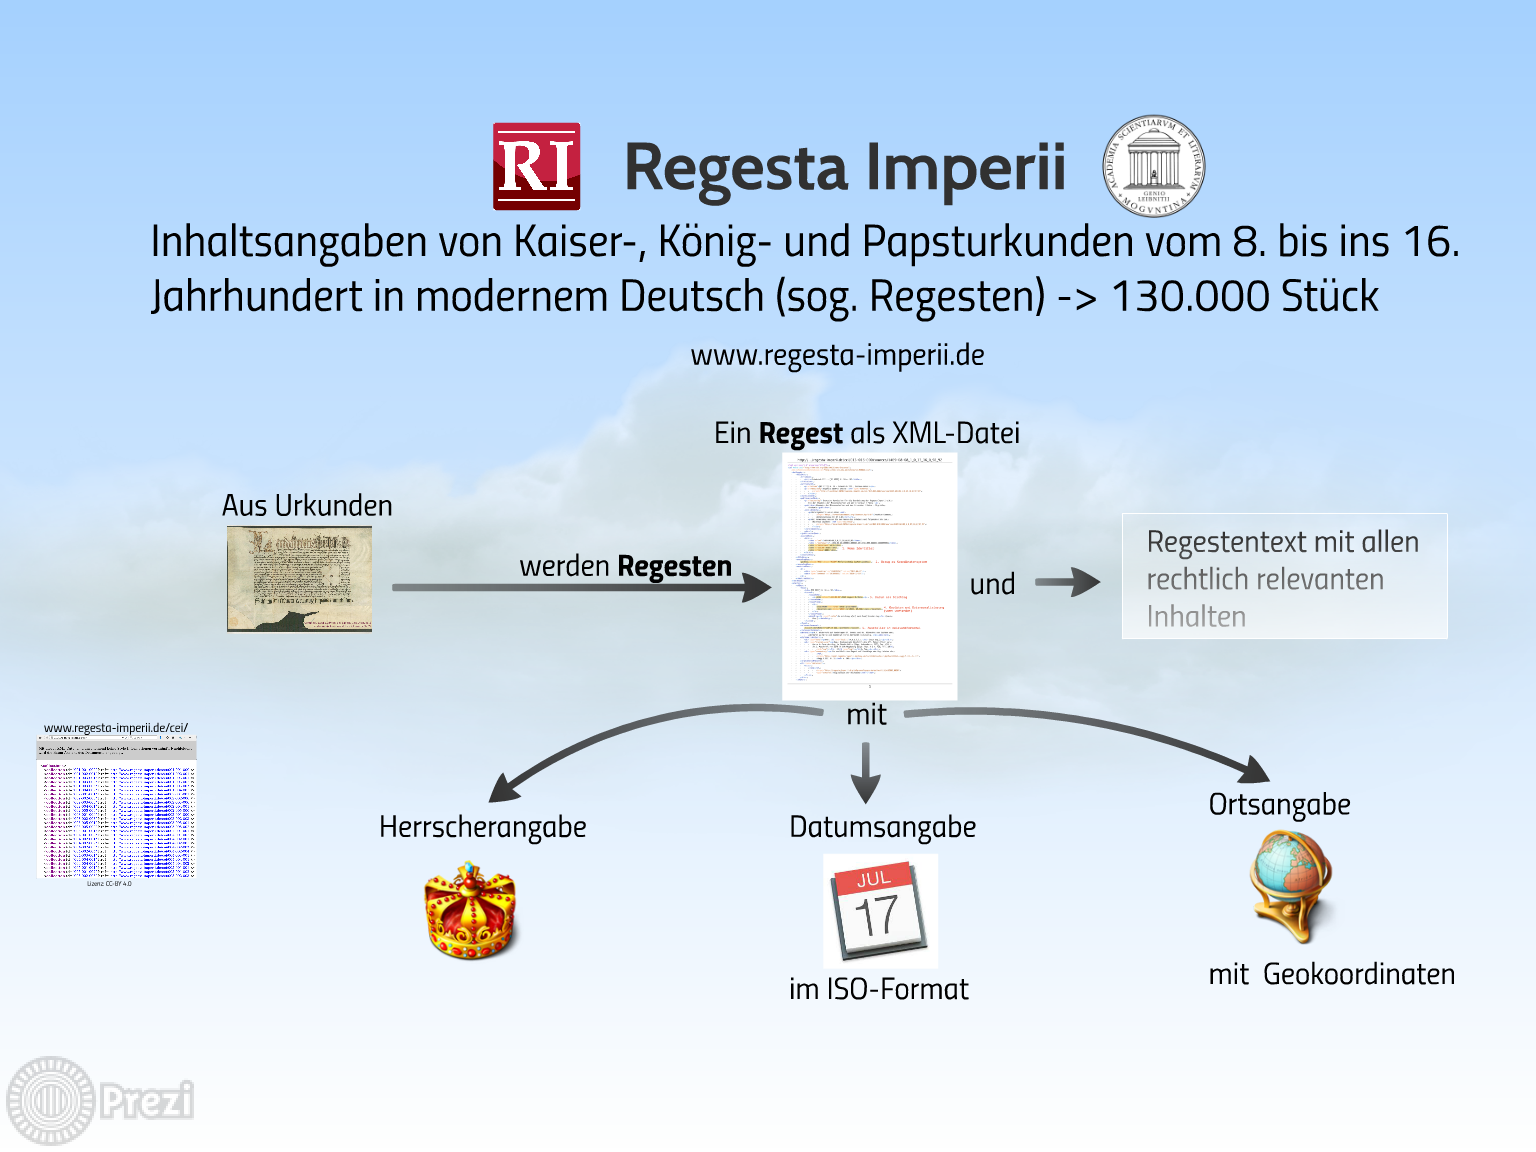
\includegraphics[width=10cm]{ri}

\end{frame}


\section{The Work}

\subsection{Data Preprocessing}

\begin{frame}[fragile]{Transformation}	% remove [fragile] if no listing
%% TODO frame %%
  All regesta XML files were transformed into a single XML file.
  \begin{itemize}
    \item
      using Python? Bash?
    \item
      some code?
  \end{itemize}
  \vspace{10 mm}
  The new XML file can be validated via XSD?
  \begin{itemize}
    \item
      some code?
  \end{itemize}
\end{frame}

\subsection{Web Application}

\begin{frame}[fragile]{Building web services}
  A web interface for searching the regesta was build.
  \begin{itemize}
    \item
      web standards + PHP
    \item
      possible to search for
      \begin{itemize}
        \item
          title
        \item
          date
        \item
          place
        \item
          issuer
      \end{itemize}
      and any combination of them of each regesta
      \begin{itemize}
        \item
          using XPath in SimpleXML
      \end{itemize}
    \item
      output with additional info/links to resources
  \end{itemize}
  \begin{lstlisting}[language=PHP]
$xml = simplexml_load_file("index.xml");

// XML: <list><document><title>...</title>...</document></list>
$document = $xml->xpath("/list/document");

foreach ($document as $node) {
    if (stripos ($node->title, $_POST['TitleInput']) > -1) { $elem[] = $pos; }
    $pos += 1;
}
  \end{lstlisting}
\end{frame}

\subsection{Additional Processing}

\begin{frame}[fragile]{XQuery}	% remove [fragile] if no listing
%% TODO frame %%
  Something for XQuery
  \begin{itemize}
    \item
      Foobar Foobar
    \item
      some code?
  \end{itemize}
  \vspace{10 mm}
  Result?
  \begin{itemize}
    \item
      something else
  \end{itemize}
\end{frame}

\begin{frame}[fragile]{SPARQL}	% remove [fragile] if no listing
%% TODO frame %%
  Something for XQuery
  \begin{itemize}
    \item
      Foobar Foobar
    \item
      some code?
  \end{itemize}
  \vspace{10 mm}
  Result?
  \begin{itemize}
    \item
      something else
  \end{itemize}
\end{frame}

\begin{frame}[fragile]{Web Services}
  Something about Web Services
  \begin{itemize}
    \item
      Foobar Foobar
    \item
      some code?
  \end{itemize}
  \vspace{10 mm}
  DBpedia?
  \begin{itemize}
    \item
      something else
  \end{itemize}
\end{frame}

\begin{frame}[fragile]{Microdata}
  \vspace{5 mm}
  Microdata was used
  \begin{itemize}
    \item
      to arrange results into pages for CSS
      \begin{lstlisting}[language=PHP]
foreach ($elem as $num) {

    if ($pos % 5 == 0) { echo '<section id="', ($pos / 5), '">'; }

    // found regesta

    if ($pos % 5 == 4) { echo '</section>'; }
    $pos += 1;
    
}
      \end{lstlisting}
    \vspace{2.5 mm}
    \item
      to insert vCards with very sensitive personal data into the website
      \begin{lstlisting}[language=HTML]
<address class="vcard">
  <span class="givenName">Numerius</span>
  <span class="familyName">Negidius</span><br>
  <a class="email" href="mailto:spam@hotmail.com">n.nescio@nn.gov</a><br>
  <span class="category">Management</span>,
  <span class="org">Freie Universität Bärlin</span>
</address>      

      \end{lstlisting}
  \end{itemize}
\end{frame}

\section{Live Demo}

\begin{frame}{Live Demo}

Let's have a look...

\end{frame}

\section*{Summary}

\begin{frame}{Summary} %% TODO (maybe) %%

  % Keep the summary *very short*.
  \begin{itemize}
  \item
    The \alert{first main message} of your talk in one or two lines.
  \item
    The \alert{second main message} of your talk in one or two lines.
  \item
    Perhaps a \alert{third message}, but not more than that.
  \end{itemize}
  
  % The following outlook is optional.
  \vskip0pt plus.5fill
  \begin{itemize}
  \item
    Outlook
    \begin{itemize}
    \item
      Something you haven't solved.
    \item
      Something else you haven't solved.
    \end{itemize}
  \end{itemize}
\end{frame}

\end{document}
